\chapter{Concepts \& Documentation}

This chapter introduces the key concepts behind the Coffee Chain ERP system and details the important documents and records used in the workflow. Understanding these concepts is essential for grasping how the ERP operates and how data flows between modules.

\section*{Key Concepts}

\subsection*{1. ERP System Integration}
The Coffee Chain ERP is designed as an integrated platform combining multiple business functions—outlet management, sales, menu management, and CRM. Integration ensures that updates in one module automatically propagate to others, reducing manual work and errors.  

\textbf{Example:} Updating a menu item in the Menu module automatically updates the Sales module, ensuring that employees sell the correct items with accurate pricing.

\subsection*{2. Module-Based Architecture}
The ERP is organized into distinct modules (containers) and components:

\begin{itemize}
    \item \textbf{Outlet Management:} Stores information about each coffee outlet, including name, location, manager, and regional manager.
    \item \textbf{Sales Module:} Handles transactions, product linking, and performance reporting.
    \item \textbf{Menu Module:} Manages products, categories, and pricing, linking to the Sales module.
    \item \textbf{CRM Module:} Tracks customer leads, interactions, and engagement metrics.
    \item \textbf{Reporting \& Analytics:} Consolidates data from all modules for dashboards and decision support.
\end{itemize}

\subsection*{3. Workflow Concepts}
\begin{itemize}
    \item \textbf{Transaction Flow:} From order placement to sales recording, each step is logged in the ERP for accuracy.
    \item \textbf{Data Synchronization:} Changes in one module (e.g., menu updates) reflect immediately in dependent modules (e.g., sales).
    \item \textbf{Decision Support:} Consolidated reports allow managers and regional managers to track KPIs such as revenue, product sales, and lead conversion rates.
\end{itemize}

\subsection*{4. User Roles and Responsibilities}
\begin{itemize}
    \item \textbf{Outlet Managers:} Manage outlet operations and ensure accurate data entry.
    \item \textbf{Regional Managers:} Compare performance across outlets and make strategic decisions.
    \item \textbf{Employees:} Enter sales and product information accurately.
    \item \textbf{Customers:} Interact with the system via orders; indirectly feed CRM data.
\end{itemize}

\subsection*{5. Concept of Containers and Components}
In this ERP context:
\begin{itemize}
    \item A \textbf{Container} represents a high-level module such as Sales, CRM, or Menu.
    \item A \textbf{Component} is a sub-part of a container that executes a specific function, e.g., the \emph{Transaction Processing Component} in Sales.
\end{itemize}

\section*{Documents in the Workflow}

\subsection*{1. Sales Records}
\begin{itemize}
    \item Captured automatically by the Sales module.
    \item Includes transaction ID, product sold, quantity, price, payment method, and timestamp.
    \item Serves as the basis for financial reports and performance analytics.
\end{itemize}

\subsection*{2. Menu Master List}
\begin{itemize}
    \item Contains all products, categories, and pricing information.
    \item Maintained in the Menu module; synchronized with Sales.
    \item Provides consistency in product offerings across outlets.
\end{itemize}

\subsection*{3. Customer \& Lead Records}
\begin{itemize}
    \item Captured by the CRM module.
    \item Includes lead source, customer information, interaction logs, and engagement metrics.
    \item Used for marketing, promotions, and improving customer relationships.
\end{itemize}

\subsection*{4. Outlet Data Sheets}
\begin{itemize}
    \item Contains outlet details: name, location, manager, regional manager.
    \item Maintained in the Outlet Management module.
    \item Supports reporting and operational oversight.
\end{itemize}

\subsection*{5. Reports and Dashboards}
\begin{itemize}
    \item Generated by the Reporting \& Analytics module.
    \item Summarizes sales, outlet performance, and customer engagement.
    \item Provides actionable insights for decision-making.
\end{itemize}

\section*{Integration of Documents with Modules}

\begin{itemize}
    \item Sales records are linked to menu items and CRM leads.
    \item Customer engagement documents feed into reporting dashboards.
    \item Outlet data is referenced for KPI calculation and performance benchmarking.
\end{itemize}

\section*{Code and Diagram Integration}

\begin{lstlisting}[language=Python, caption={Example: Sales Transaction Recording in Python}]
class SaleOrder(models.Model):
    _inherit = 'sale.order'

    outlet_id = fields.Many2one('coffee.outlet', string='Outlet')
    customer_id = fields.Many2one('res.partner', string='Customer')
\end{lstlisting}

\begin{figure}[H]
\centering
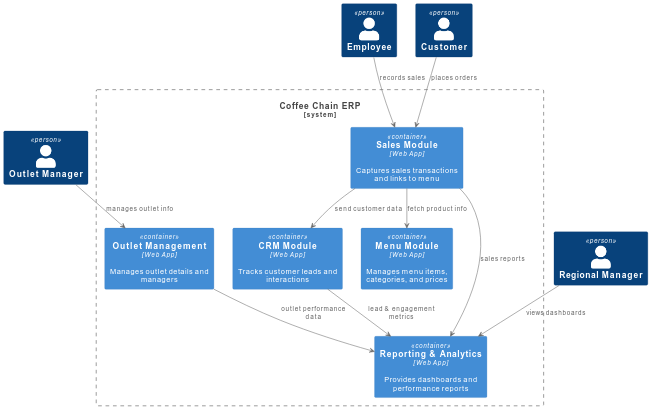
\includegraphics[width=0.9\textwidth,keepaspectratio]{diagrams/C2.png}
\caption{Reference Container Diagram for Document Flow}
\end{figure}

\section*{Insights}

\begin{itemize}
    \item Centralizing document management reduces errors and ensures data consistency.
    \item Clear linkage between documents and modules enhances traceability and decision-making.
    \item Automated capture of sales, menu, and customer data minimizes manual intervention.
    \item Reporting dashboards serve as the single source of truth for management insights.
\end{itemize}
